\subsection{L'intelligence artificielle au service de la génomique comparée}

\subsubsection{Définitions et concepts}

Avec l’accumulation massive de données, la génomique est désormais confrontée aux défis du \textit{Big Data}, tant en termes de volume que de complexité. Les bioinformaticiens se tournent donc vers des méthodes développées dans la science des données (\textit{data science}) et particulièrement vers l'intelligence artificielle (IA). L’intelligence artificielle regroupe un ensemble de techniques permettant aux machines de reproduire certaines facultés cognitives humaines, telles que l’apprentissage, le raisonnement et la résolution de problèmes. Elle s’appuie sur divers domaines de recherche définissant le traitement des données, la prise de décision et l’adaptation des algorithmes aux informations reçues. Ici, nous nous intéresserons à un champ de recherche particulièrement utilisé en bioinformatique, celui de l'apprentissage automatique (\textit{machine learning en anglais}, ML). 

Les méthodes de ML correspondent à des méthodes qui s'améliorent par l'apprentissage ou l'entraînement. Pour fonctionner, elles ont besoin de grands jeux de données, bien définis. Elles sont donc bien adaptées à la génomique du Big Data. Dans une application de ML (\autoref{fig:ML_base}), après avoir bien défini les données d'entrée et la prédiction attendue, une phase d'apprentissage permet de construire le modèle le plus adapté. La première étape de l'apprentissage consiste à entraîner le modèle sur un jeu de données (d’entraînement) pour sélectionner les caractéristiques les plus pertinentes et estimer les meilleurs paramètres du modèle. Une deuxième étape d'évaluation (ou de test) mesure les performances du modèle, \textit{i.e.}, la divergence avec le résultat attendu\footnote{Cette divergence est mesurée par la fonction de perte ou de coût}. En fonction de l'évaluation, un nouvel apprentissage peut être relancé pour améliorer le modèle. Même si le modèle ne sera jamais idéal, le choix des jeux d’entraînement et de test permet de s'approcher au mieux de la prédiction souhaitée. 

\begin{figure}[htbp]
    \centering
    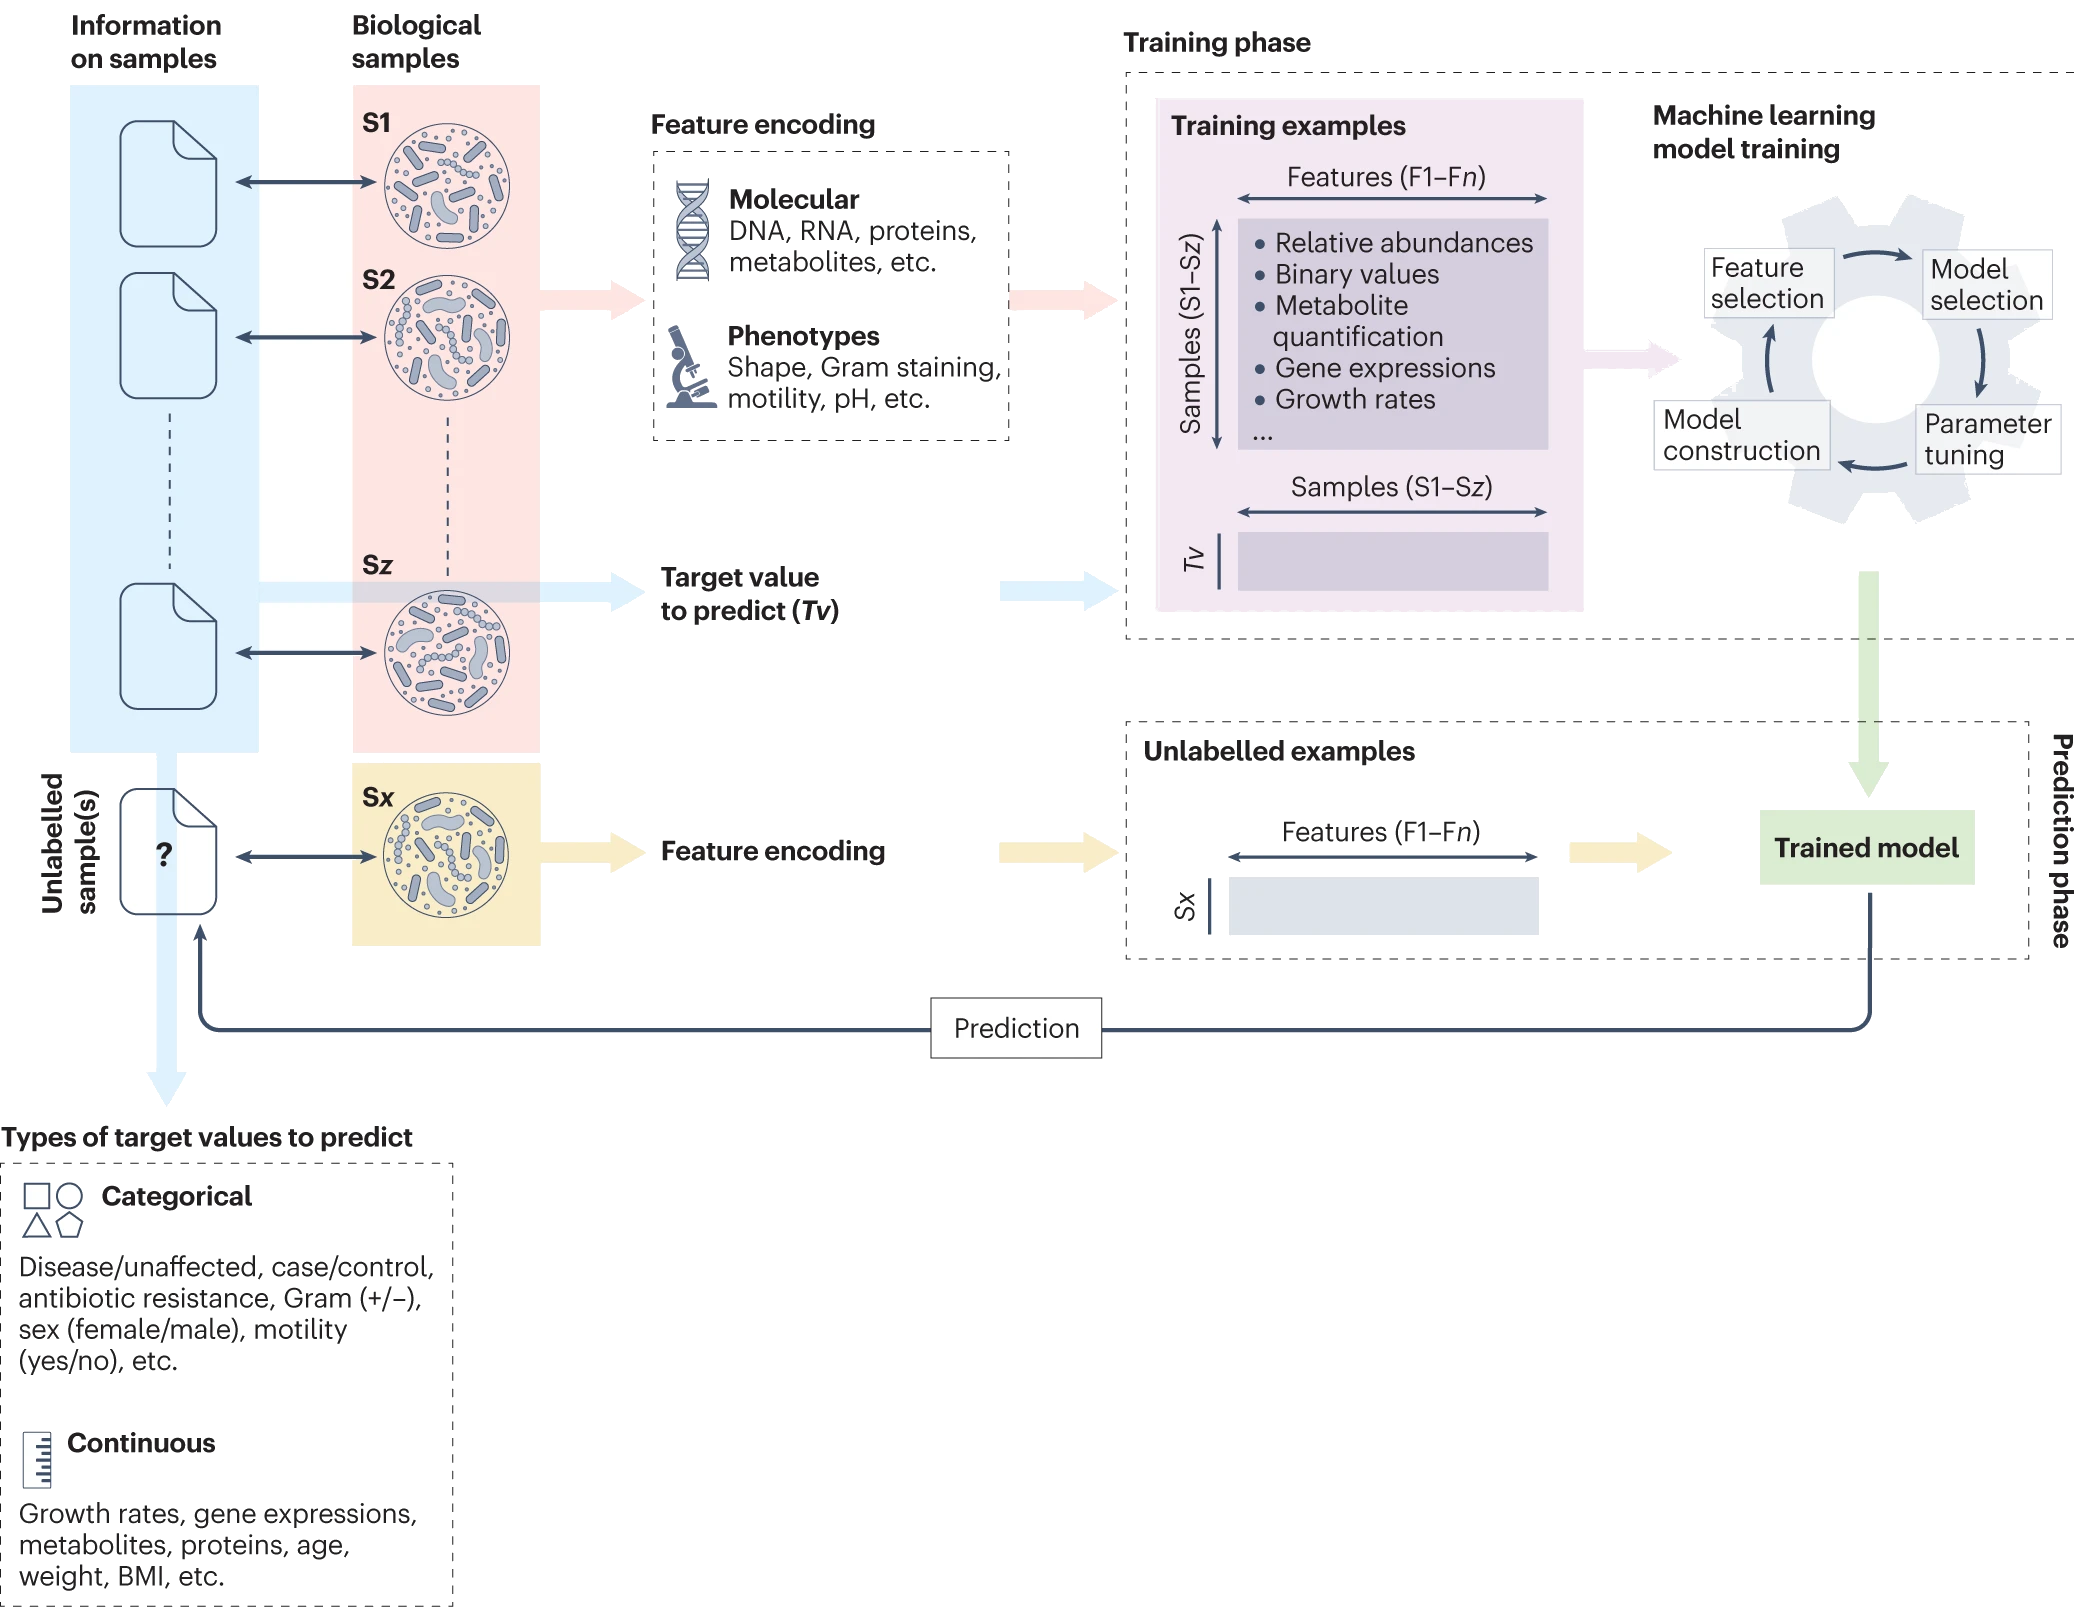
\includegraphics[width=\linewidth]{images/ML.png}
    \caption[Schéma général d'une application de machine learning]{\textbf{Schéma général d'une application de machine learning pour l'assignation de caractéristiques moléculaires et phénotypiques.} Le schéma correspond à l'application d'un modèle supervisé où les données d'entrée sont étiquetées et dont la prédiction attendue est, elle aussi, une étiquette. Extrait de \cite{asnicar_machine_2024}}
    \label{fig:ML_base}
\end{figure}

\newpage

Les méthodes de machine learning peuvent être divisées en 2 grandes catégories : (\textit{i}) l'apprentissage \textbf{supervisé}; (\textit{ii}) l'apprentissage \textbf{non supervisée}. 

Les modèles supervisés permettent d'assigner des \textbf{étiquettes} aux données. Dans ce cas, les données du jeu d’entraînement et de test sont étiquetées par le résultat attendu (à priori). La \autoref{fig:ML_base}, présente un ensemble d'échantillons dont on possède les informations d'intérêt. Le modèle entraîné est appliqué sur un nouvel échantillon et permet donc de prédire les informations jusqu'alors inconnues. Par exemple, en entraînant un classificateur supervisé (tel qu’un modèle de régression) sur des assignations génome-espèce connues, et en utilisant la présence ou l’absence de gènes marqueurs comme caractéristiques, il devient possible d’attribuer une taxonomie à un nouveau génome.

Les modèles non supervisés permettent de rechercher des structures dans des données sans nécessité d'étiquettes. Dans ce cas, après la phase d’entraînement, il y a une autoévaluation du modèle basée sur un renforcement positif. Par exemple, si l'on s'intéresse aux gènes impliqués dans la croissance bactérienne, les modèles peuvent partitionner les groupes de gènes présentant des profils d'expression génique similaires reflétant la croissance cellulaire. Les modèles non supervisés ont l'intérêt de pouvoir résoudre des problèmes plus complexes, sans avoir besoin de données annotées ; par contre, ils sont beaucoup plus imprévisibles que les modèles supervisés.

\begin{figure}[htbp]
    \centering
    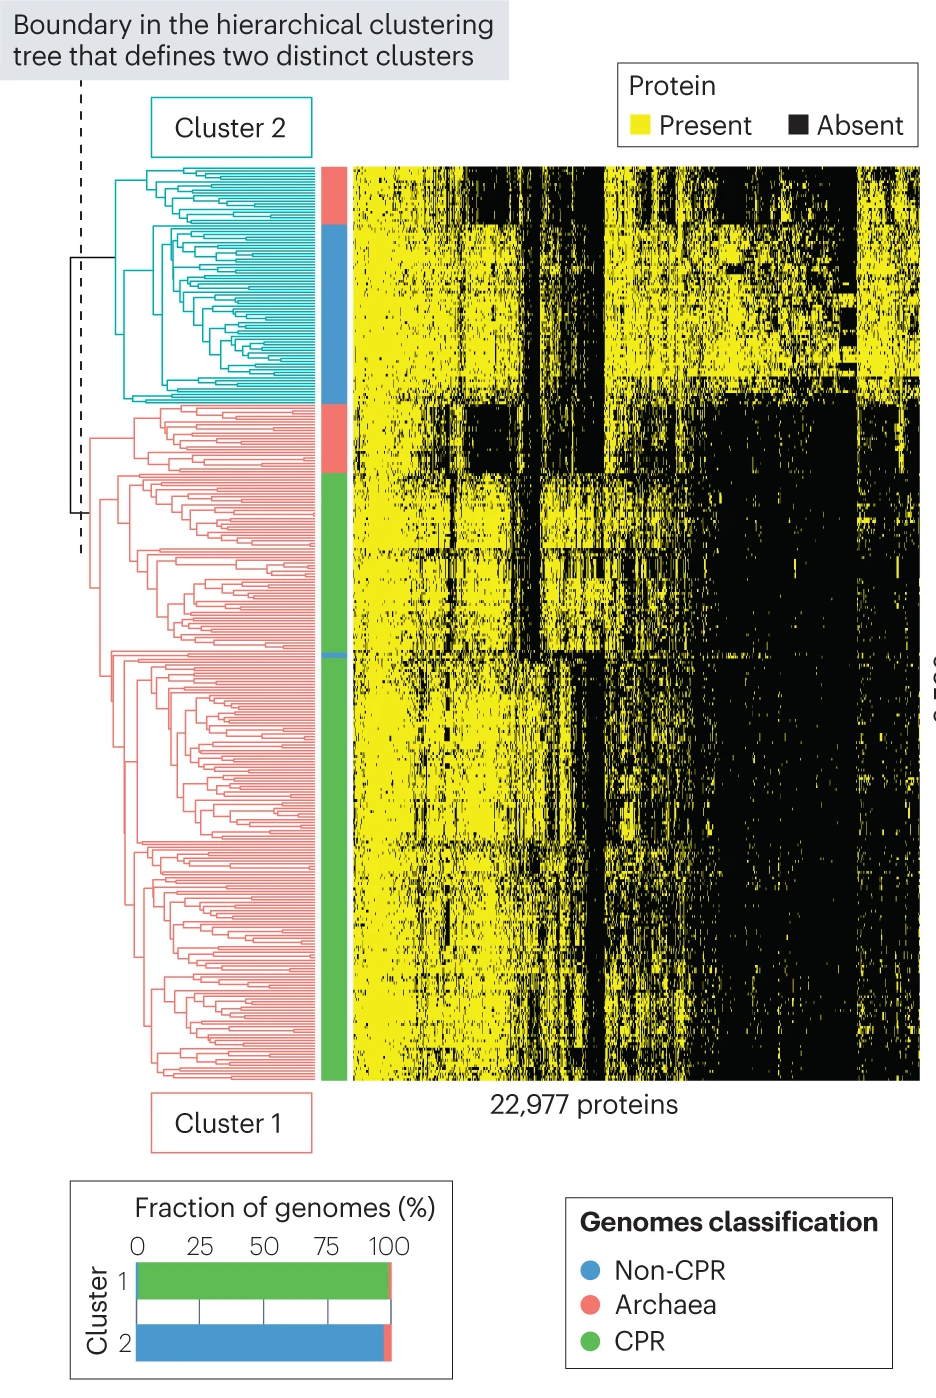
\includegraphics[width=0.5\linewidth]{images/hierachical_clustering.png}
    \caption[Exemple d'application de méthode non supervisé]{\textbf{Exemple d'application de méthode non supervisée.} Le \textit{HeatMap} représente pour chaque souche la présence/absence d'un ensemble de protéines. La méthode de clustering (ici une Analyse en composantes principales) permet d'identifier 2 groupes dans les souches, correspondant à 2 groupes taxonomiques. Extrait et adapté de \cite{asnicar_machine_2024}}
    \label{fig:enter-label}
\end{figure}

Dans les années 2010, un sous-domaine de l'apprentissage automatique gagne en popularité, l'apprentissage profond (\textit{deep learning} en anglais DL)\footnote{Les premières approches de DL datent des années 1940. Le terme regagne en popularité en 2006 suite à l'article de Geoffrey Hinton and Ruslan Salakhutdinov \cite{hinton_fast_2006}}. Les algorithmes de DL sont basés sur le concept de \textbf{réseaux neuronaux} (artificiels). Ces réseaux peuvent être représentés sous forme d'un graphe orienté, pondéré et étiqueté, comme sur la \autoref{fig:reseaux}. Ce réseau est organisé en couches successives, avec une couche d'entrée (à gauche) correspondant aux données brutes, des couches cachées (au centre) qui effectuent des transformations des données et extraient des caractéristiques, et enfin une couche de sortie (à droite) qui contient la prédiction. L'intérêt du DL réside dans sa capacité à extraire automatiquement les caractéristiques pertinentes lorsque les données passent dans les couches cachées. Plus le nombre de couches est élevé, plus le modèle peut apprendre, plus les questions que l'on pose peuvent être complexes et les réponses précises. Cependant, en augmentant la complexité, on augmente aussi la difficulté d'interprétation\footnote{On parle parfois de boite noire dans les modèles les plus complexes dans le sens où, dans les couches cachées, il est souvent difficile de savoir comment les données ont été transformées et classées.}. 

\begin{figure}
    \centering
    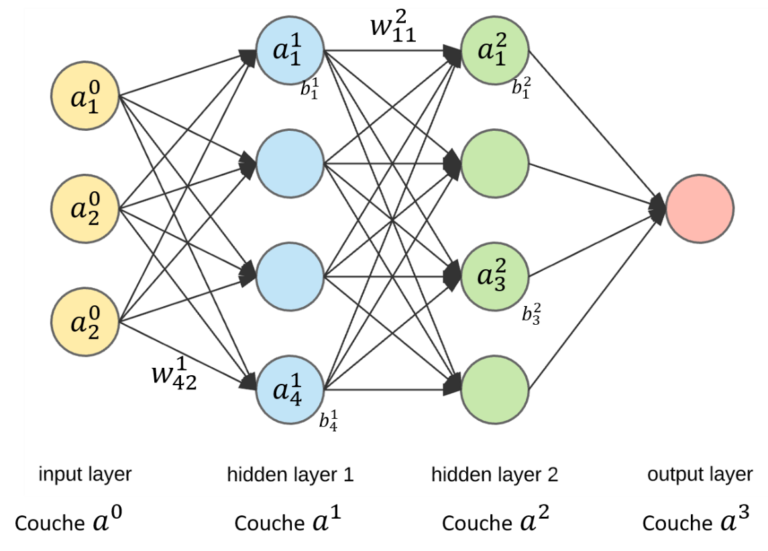
\includegraphics[width=0.5\linewidth]{images/reseaux_neurone.png}
    \caption[Représentation d'un réseau de neurone à 3 couches]{\textbf{Représentation d'un réseau de neurones à 3 couches.} Extrait de \url{https://www.aspexit.com/reseau-de-neurones-on-va-essayer-de-demystifier-un-peu-tout-ca-1/}}
    \label{fig:reseaux}
\end{figure}

Réaliser une étude de ML/DL peut être un problème épineux. Il faut d'abord avoir une bonne compréhension des données pour s'orienter vers des méthodes supervisées ou non, et choisir entre l'apprentissage traditionnel et profond (cf. \autoref{tab:ML_met} 
\& \autoref{tab:dl_met}). Il convient également de s'assurer de la qualité des données ; si le modèle apprend sur des données corrompues, les prédictions seront fausses. Ceci fait, on choisit un modèle et des paramètres, dont on évalue les performances. L'indicateur doit être choisi judicieusement pour refléter correctement l'efficacité du modèle. L'évaluation du modèle doit aussi être reproductible, \textit{i.e.} testée sur de nouveaux jeux de données via des approches comme la validation croisée entre ensembles distincts. Un autre point d'attention est celui du sur-apprentissage (\textit{overfitting} en anglais). Un modèle trop complexe risque de capturer non seulement les relations sous-jacentes, mais aussi le bruit des données, menant ainsi à des résultats biaisés. Tous ces points sont suffisamment importants pour que finalement "Le choix d'un algorithme d'apprentissage automatique particulier [est] moins important que son application et son utilisation correctes et différents algorithmes d'apprentissage automatique appliqués de la bonne manière devraient fournir des résultats cohérents." \cite{asnicar_machine_2024}.

\begin{table}[htbp]
    \centering
    % \footnotesize
    \small
    \begin{sideways}
    \begin{tabular}{|>{\raggedright\arraybackslash}p{0.1\textheight}|>{\raggedright\arraybackslash}p{0.1\textheight}|>{\raggedright\arraybackslash}p{0.15\textheight}|>{\raggedright\arraybackslash}p{0.275\textheight}|>{\raggedright\arraybackslash}p{0.275\textheight}|}
    \hline
    \textbf{Méthode} & \textbf{Type de données} & \textbf{Exemples d'applications} & \textbf{Avantages} & \textbf{Inconvénients} \\
    \hline
    Régression Ridge (et LASSO / élastique) & \multirow{5}{0.1\textheight}[-5em]{Étiquetées Nombre de caractéristiques fixe} & Prédiction de l'expression des gènes en réponse à des antibiotiques & Facile à interpréter \newline Facile à entraîner \newline Bon benchmark & Ne peut pas apprendre des relations complexes entre caractéristiques \newline Sur-apprend avec un grand nombre de caractéristiques \\
    \cline{1-1}\cline{3-5}
    Machine à vecteurs de support & & Classification des gènes en fonction de leur fonction & Peut effectuer à la fois la classification et la régression linéaire et non linéaire & Difficile à adapter à de grands ensembles de données \\    
    \cline{1-1}\cline{3-5}
    Forêt aléatoire &  & Identification des mutations génomiques associées à un phénotype & Apprend l'importance de chaque caractéristique pour la prédiction \newline Les arbres de décision individuels sont lisibles par l'humain \newline Moins sensible à l'échelle et à la normalisation des caractéristiques, donc plus facile à entraîner et à ajuster & Moins approprié pour la régression \newline De nombreux arbres de décision sont difficiles à interpréter \\     
    \cline{1-1}\cline{3-5}
    Boosting de gradient (ex. XGBoost) & & Profilage de l'expression des gènes & Apprend l'importance de chaque caractéristique \newline Arbres de décision lisibles par l'humain Moins sensible à l'échelle et à la normalisation & Peut avoir du mal à apprendre le signal sous-jacent en présence de bruit Moins adapté à la régression \\
    \hline
    Clustering & Non étiquetées \newline Nombre de caractéristiques fixe & Groupement des gènes bactériens en fonction de leurs profils d'expression dans différentes conditions environnementales & Bon clustering facilement identifiable pour les données de faible dimension \newline Métriques de validation de clustering disponibles & Difficile à appliquer à de grands ensembles de données \newline Les ensembles de données bruités peuvent produire des résultats contradictoires \\     
    \hline
    Réduction de dimensionnalité & Non étiquetée Grand nombre de caractéristiques fixe & Visualisation des relations entre différentes souches bactériennes basées sur leurs génomes & Fournit une représentation visuelle des données Évaluations de l'ajustement souvent disponibles & Difficile de préserver à la fois les différences locales et globales Difficile à appliquer à un grand nombre d'échantillons \\        
    \hline
    \end{tabular}
    \end{sideways}
    \caption[Méthodes de Machine learning]{\textbf{Méthodes de Machine learning.} Extrait et adapté de \cite{greener_guide_2022}}
    \label{tab:ML_met}
\end{table}

\begin{table}[htbp]
    \centering
    \small
   \begin{sideways}
   \begin{tabular}{|>{\raggedright\arraybackslash}p{0.1\textheight}|>{\raggedright\arraybackslash}p{0.1\textheight}|>
   {\raggedright\arraybackslash}p{0.2\textheight}|>{\raggedright\arraybackslash}p{0.25\textheight}|>{\raggedright\arraybackslash}p{0.25\textheight}|}
    \hline
    \textbf{Méthode} & type de données & \textbf{Exemples d'applications} & \textbf{Avantages} & \textbf{Inconvénients} \\
    \hline
    Réseau de neurones convolutionnel (CNN) & Données spatiales disposées dans une grille \newline Permet une taille d'entrée variable & Identification des motifs régulateurs dans les séquences d'ADN bactérien & Taille d'entrée variable Apprend des motifs indépendamment de leur localisation & Champ réceptif limité Difficile à entraîner pour des architectures profondes \\
    \hline
    Perceptron multicouche & Étiqueté \newline Nombre fixe de caractéristiques& Prédiction des interactions protéine-protéine & Moins de couches nécessaires que les CNN, donc plus rapide et plus facile à entraîner & Facile à sur-apprendre Grand nombre de paramètres Difficile à interpréter \\
    \hline
    Réseau de neurones récurrent (RNN) & Données séquentielles \newline Permets une taille d'entrée variable & Prédiction des séquences d'ARN non codant fonctionnel chez les procaryotes & Taille d'entrée variable Les séquences sont fréquentes en biologie & Long temps d'entraînement \newline Exige beaucoup de mémoire \\
    \hline
    Réseau de neurones convolutionnel sur graphe (GCN) & Données caractérisées par des connexions entre entités \newline Permets une taille d'entrée variable & Modélisation des interactions entre protéines dans les complexes multiprotéiques bactériens & Modélise les interactions complexes Flexible pour différents types de relations & Difficile à interpréter \newline Peut être exigeant en termes de calcul \\
    \hline
    Autoencodeurs & Données étiquetées ou non \newline Taille d'entrée fixe ou variable & Ingénierie des protéines et des gènes \newline
    Prédiction de la méthylation de l'ADN & L'espace latent fournit une représentation à faible dimension qui peut être utilisée pour visualiser les données d'entrée \newline Peut générer de nouveaux échantillons, ce qui est utile dans des domaines tels que la conception de protéines & Espace latent spécifique aux données de l'ensemble d'entraînement et peut ne pas être approprié à d'autres ensembles de données \newline Le test des échantillons nouvellement générés nécessite souvent des expériences en laboratoire humide \\
    \hline
    \end{tabular}
   \end{sideways}
    \caption[Méthode de deep learning]{\textbf{Méthodes de Deep Learning.} Extrait et adapté de \cite{greener_guide_2022}}
    \label{tab:dl_met}
\end{table}

\newpage

\subsubsection{Application de la génomique comparée pour l'étude des procaryotes}

L'application des méthodes de ML à l'étude des génomes procaryotes a permis d'améliorer l'identification et l'annotation des séquences génétiques, notamment grâce à la capacité des algorithmes ML à reconnaître des motifs complexes et à traiter de grandes quantités de données. Plusieurs outils exploitant ces techniques ont émergé, chacun se concentrant sur des aspects spécifiques de l'analyse génomique.

Nucleic Transformer \cite{he_nucleic_2023} est un outil basé sur l'apprentissage profond conçu pour l'analyse et la classification des séquences d'acides nucléiques. Il utilise une combinaison de mécanismes d'\textbf{auto-attention} et de \textbf{convolutions} pour identifier des motifs complexes dans l'ADN et l'ARN. L’auto-attention permet au modèle de capturer des relations à longue distance entre les bases nucléiques, tandis que les convolutions sont efficaces pour détecter des motifs locaux récurrents. Son architecture permet d'analyser de grands ensembles de données génomiques tout en maintenant une précision élevée. L’une des analyses réalisables avec Nucleic Transformer est l'identification des promoteurs bactériens. Dans l'article de He \textit{et al.}, Nucleic Transformer est entraîné et testé sur un jeu de données de 5 720 séquences, dont la moitié sont des promotrices. Les prédictions du modèle surpassent celles des outils classiques d'environ 2 \%. D'autres applications sont possibles, comme classifier des génomes viraux ou identifier des éléments régulateurs dans les génomes, facilitant ainsi l'étude des réseaux de régulation et des adaptations microbiennes.

ResFinder\cite{zankari_identification_2012} est un outil initialement développé sans modèle de ML. ResFinder fournissait une base de données de gènes de résistance aux antibiotiques et les séquences étaient alignées (avec BLAST) sur cette base de données. Dans sa version 4.0 \cite{bortolaia_resfinder_2020}, il intègre la notion de combinaisons entre des résistances et des espèces bactériennes. Cette méthode permet d'obtenir des prédictions fiables pour les organismes et les gènes de résistance bien connus. Cependant, pour ceux qui sont moins étudiés, les prédictions sont moins précises. En 2022, ResFinder intègre des méthodes de ML pour combler ce manque \cite{florensa_resfinder_2022}. Grâce à des algorithmes d’apprentissage supervisé, il peut identifier des signatures génétiques associées à des résistances spécifiques. L’avantage principal de ResFinder réside dans sa DB de haute qualité, garantissant un apprentissage fiable des modèles. D'autres méthodes utilisaient déjà des modèles de ML pour identifier les gènes de résistance, par exemple le modèle de classification \textit{Random-forest} \cite{aytan-aktug_predicting_2021}, ou des réseaux de neurones \cite{aytan-aktug_prediction_2020}.


Kaiju \cite{menzel_fast_2016} est un classificateur taxonomique qui utilise des approches de machine learning pour identifier rapidement des microorganismes à partir de données métagénomiques. Contrairement aux méthodes d’alignement classiques, il repose sur une approche fondée sur les k-mers et des techniques de classification, ce qui lui permet d’annoter efficacement des séquences, y compris lorsqu’elles sont courtes et fragmentées. Kaiju exploite des structures algorithmiques avancées, notamment la Burrows-Wheeler Transform (BWT), qui réorganise les séquences pour optimiser la recherche rapide de motifs, et les Maximums Exact Matches (MEMs), qui détectent les plus longues sous-séquences exactes partagées entre un fragment et une base de référence. Ces méthodes permettent d’accélérer l’identification des séquences en comparant directement les fragments d’ADN à une base de données de génomes de référence. Cette stratégie réduit le besoin d’alignement global, rendant l’analyse plus rapide et plus adaptée pour de grands volumes de données. Grâce à cette architecture hybride combinant algorithmes efficaces et modèles d’apprentissage, Kaiju est particulièrement adapté à l’analyse d’échantillons environnementaux et cliniques.


LookingGlass \cite{hoarfrost_deep_2022} est un outil utilisant des modèles de DL pour capturer la complexité des relations fonctionnelles et phylogénétiques entre les séquences grâce à une architecture de type réseau de neurones récurrents à mémoire longue et courte (LSTM). Ce type de réseau neuronal est particulièrement adapté aux données séquentielles comme l’ADN, car il permet de modéliser des dépendances à long terme en conservant en mémoire des informations clés sur de longues distances dans la séquence. En exploitant l’apprentissage non supervisé, le modèle est capable d’identifier des relations évolutives au-delà des similarités de séquence directes, permettant ainsi la reconnaissance de fonctions moléculaires dans des séquences non annotées. LookingGlass intègre aussi de l'apprentissage par transfert, \textit{i.e.} qu'il peut transférer l'apprentissage acquis sur une prédiction à d'autres prédictions. LookingGlass a été éprouvé sur l'identification de nouvelles oxydoréductases, la prédiction de températures optimales d’enzymes, ou encore la détection des cadres de lecture dans des fragments d’ADN courts. Cette approche permet également d'étudier une partie inexplorée de la diversité microbienne, \textit{i.e.} les séquences non caractérisées qui constituent la majeure partie du monde microbien (\textit{microbial dark matter}). LookingGlass ouvre ainsi la voie à une annotation plus rapide et plus exhaustive des métagénomes, facilitant la compréhension des réseaux fonctionnels microbiens et leur impact sur les écosystèmes et la santé humaine.

Les outils de prédiction des systèmes de défense contre les phages bénéficient aussi des développements des modèles d'apprentissage. L'outil CRISPRidentify\cite{mitrofanov_crispridentify_2021} commence par identifier les séquences CRISPR candidates. La seconde phase, extrait différentes caractéristiques parmi les candidates (stabilité des ARNcr, similarité avec les CRISPRs connus, tailles des \textit{spacers}\dots, contenu en nucléotide AT). Enfin, un algorithme de classification, basé sur le modèle ExtraTrees, permet de valider et d'assigner un score de confiance aux candidates. Ce modèle d'apprentissage automatique repose sur un ensemble d'arbres de décision construits de manière aléatoire et indépendante, optimisant ainsi la robustesse et la précision des prédictions. Comparé aux autres outils de détection CRISPR, CRISPRidentify est plus sensible et retourne moins de faux positifs. D'autres outils, comme DeepDefense \cite{hauns_deepdefense_2024} et DeepPredictor\cite{hauns_deepdefense_2024} utilisent des méthodes de \textit{deeplearning}, pour la prédiction de systèmes de défense. L'intérêt de ces méthodes basé sur l'apprentissage machine est qu'elles détectent plus de systèmes et même des systèmes inconnus. Toutefois, ces méthodes sont très sensibles aux données d'apprentissage. De plus, elles demandent beaucoup de ressources de calcul, et notamment, dans les exemples présentés, le nombre de génomes utilisés reste plutôt limité par rapport au nombre de génomes disponibles dans les banques.